%!TEX root = ../doc.tex
\chapter{Konzept}
\label{sec:konzept}

Aus den Anforderungen ist klar ersichtlich dass eine eigene Benutzeroberfläche entwickelt werden soll, welche über die Programmierschnittstelle von LoBo kommunizieren soll. Die nicht funktionelle Anforderung NFREQ-001 verlangt eine Web Browser kompatible Benutzeroberfläche und disqualifiziert eine zu installierende Desktop Client Anwendung. Trotz der Limitierung der Lösungsmöglichkeiten, bleiben bei der Entwicklung einer Benutzeroberfläche im Web viele Fragen offen. Im folgenden werden die Technologie- sowie Architekturentscheidungen vorgestellt und begründet.

\section{Web Modell}
Traditionelle Websites bestehen aus mehreren \textit{Hyper Text Markup Language} (HTML) Seiten und liefern diese, wenn der Client sie anfordert aus. Es gibt verschiedene Programmiersprachen welche es erlauben zum Zeitpunkt des Aufrufs, Code welcher in diesen HTML Seiten vorhanden ist zu interpretieren und des entsprechende Resultat auszuliefern. \textit{PHP Hypertext Preprocessor}\footnote{Offizielle Website von PHP: \url{http://php.net/}} (PHP) ist eine der bekanntesten Programmiersprachen. Aber auch Python bietet mit dem Framework \textit{Django}\footnote{Offizielle Website von Django: \url{https://www.djangoproject.com}} eine ähnliche Funktionalität an. Mit der zunehmende Möglichkeiten im Web sowie der immer grösseren Komplexität wurden andere Modelle für das Web entwickelt. Mit der offiziellen Spezifikation des \textit{XMLHttpRequest Object} am 5. April 2006\citep[]{w3cXMLHttpRequest} und dessen Einsatz von Google in Webapplikationen wie Gmail und Google Maps, wurde die Entwicklung von \textit{Single-page application} (SPA) ermöglicht. Mit \textit{XMLHttpRequest} ist es möglich nach dem Laden der Website eine Anfrage an den Server zu schicken ohne dabei die Gesamte HTML Seite neu zu laden. Für die Ausführung dieser \textit{XMLHttpRequest} Anfragen wird eine clientseitige Skriptsprache benötigt. Trotz vereinzelten Alternativen ist JavaScript der Standard bei den browserfähigen clientseitigen Skriptsprachen. Dies ist mitunter auch ein Grund warum SPA Webseiten mit JavaScript erstellt werden. In den Abbildungen  \ref{fig:requestHtml} und \ref{fig:requestXHtml} \footnote{Bilder von \url{https://blog.4psa.com/an-intro-into-single-page-applications-spa/}} ist der Unterschied zwischen einer konventionellen Website und einer SPA veranschaulicht.

\begin{figure}[ht]
	\centering
  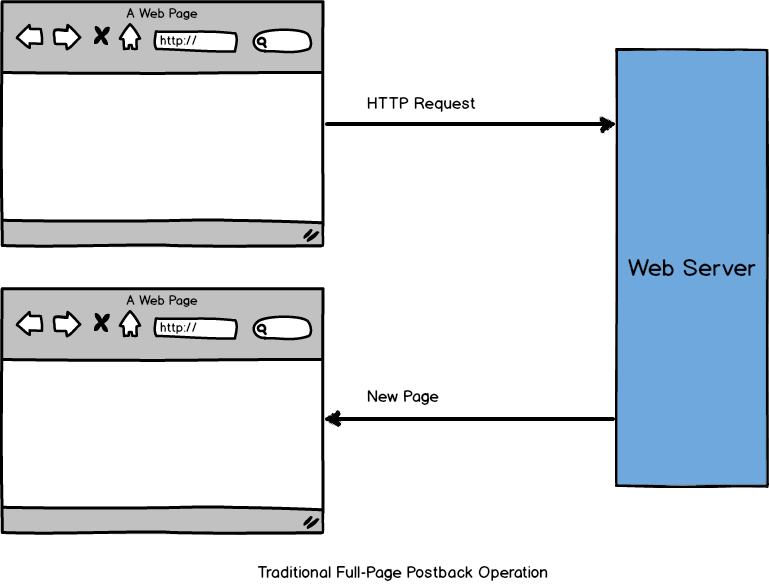
\includegraphics[width=0.88\textwidth]{images/requestHtml.png}
	\caption{Visualisierung einer Anfrage in einer konventionellen Webseite}
	\label{fig:requestHtml}
\end{figure}

\begin{figure}[ht]
	\centering
  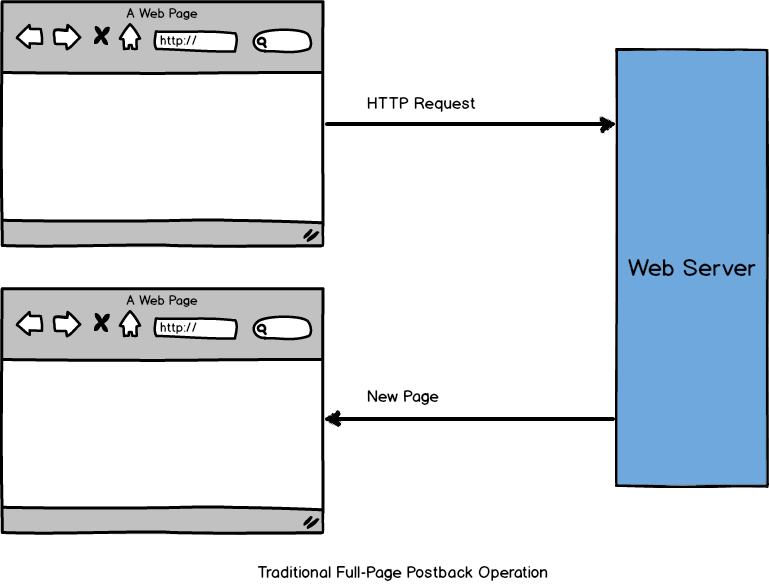
\includegraphics[width=0.88\textwidth]{images/requestHtml.png}
	\caption{Visualisierung einer Anfrage in einer Single-page Applikation}
	\label{fig:requestXHtml}
\end{figure}


\subsection{Single-page application}
\textit{Single-page application} (SPA) haben viele Vorteile gegenüber traditionellen Webseiten. Die Gesamte Webseite kann mit wenigen Anfrage an den Server geladen werden. Im wesentlichen werden nur drei Anfragen (1. HTML Seite, 2. Cascading Style Sheets (CSS), 3. JavaScript) benötigt. Alle weiteren Daten wie z.B. Benutzerdaten aus der Datenbank werden asynchron mit einer \textit{XMLHttpRequest} Anfrage, während die Webseite im Browser aufgebaut wird, geladen. Dies hat den Vorteil dass die Webseite bedeutend schneller geladen wird und trägt damit zur Benutzerfreundlichkeit bei. Im folgende ist eine nicht abgeschlossene Liste mit den Vorteilen von SPA.
\begin{description}
	\item[Entlastung] Die Benutzeroberfläche wird komplett im Browser erstellt und benötigt dafür keine Ressourcen vom Server.
	\item[Entkopplung] Daten und Businesslogik sind nicht mehr an die Visuellen Elemente gebunden.
	\item[Performant] Single-page Applikationen verwalten ihren eigenen Status und benötigten dafür weniger Informationen vom Server.
\end{description}
SPA setzten voraus dass der Server ein definierte Schnittstelle besitzt über welche Daten geladen bzw. geschrieben werden können. Dies hat zusätzlich der Vorteil, dass auch Applikationen anderer Plattformen wie z.B. Android oder iOS auf diese Schnittstellen zugreifen können.
\newline{}
Ein grosser Nachteil von Single-Page Applikationen ist die Lesbarkeit des auszuführenden Codes. JavaScript ist eine Skriptsprache welche zur Laufzeit interpretiert und ausgeführt wird. Dies bedeutet dass der gesamte Code im Browser vorhanden ist und für den Benutzer lesbar ist. Es gibt Werkzeuge welche diesen Code versuchen unleserlich zu machen in dem Variablen umbenennt und Leerzeichen entfernt werden, aber mit Energie und Geduld kann auch dies wieder lesbar gemacht werden.

\subsection{Mini-Backend}
Für die Auslieferung der \textit{Single-page application} wird nur ein Webserver wie z.B. Apache\footnote{Apache ist ein weitverbreiteter opensource Webserver \url{https://httpd.apache.org/}} oder Nginx benötigt. Die SPA kann aber auch von einem Webserver ausgeliefert werden, welcher eigene Logik besitzt. Im Rahmen dieser Bachelorarbeit nenne ich die Benutzung eines Webservers mit eigener Logik Mini-Backend. Es existieren mehrere Plattformen in verschiedenen Programmiersprachen mit welchen die Entwicklung eines Mini-Backend möglich wäre.  Node.js\footnote{Node.js ist eine Serverseitige Plattform \url{https://nodejs.org}} ist eine serverseitige Plattform welche auf JavaScript basiert und die Möglichkeit bietet Webseiten auszuliefern und eigene Logik auszuführen. Diese Logik bzw. dieser Code befindet sich immer auf dem Server und kann von den Benutzer nicht gelesen werden. Node.js kann die gesamte Businesslogik eines Projektes beinhalten oder aber nur Webanfragen weiterleiten

\subsection{Fazit}
Obwohl die Logik für die zu entwickelnde Benutzeroberfläche ausschliesslich in der SPA ausgeführt werden könnte, hat der Einsatz eines sogenannten Mini Backends erhebliche Vorteile. LoBo benutzt für die Authentifizierung einen Schlüssel mit welchem alle Anfragen \textit{gehasht} werden müssen. Der Entstandene Hash wird im Header jeder Anfrage mitgeschickt. Dadurch kann LoBo die Authenzität und Integrität der Anfragen sicher stellen. Dieses hashing könnte in der SPA geschehen, hat jedoch den Nachteil, dass der Schlüssel von den Benutzer ausgelesen werden kann. Zusätzlich vereinfacht der Einsatz eines Mini-Backend die Skalierung. Es können mehrere Instanzen des Mini-Backends gestartet werden und ein zusätzlicher Webserver verteilt die Anfragen auf die verfügbaren Instanzen. Die Mini-Backends können auch mit verschiedenen LoBo Systemen kommunizieren. Dies verhindert einen Flaschenhals bei einem Anstieg der Benutzerzahlen. Im Rahmen dieser Bachelorarbeit wird eine Single-page Applikation mit JavaScript entwickelt und ein Mini-Backend welches auf Node.js basiert. Node.js wurde ausgewählt weil es in der gleichen Sprache programmiert wird, wie die SPA und dadurch einige Vorteile bietet.

\section{JavaScript}
JavaScript ist zurzeit eine der populärsten Programmiersprachen. Die Sprache hat im Juni 2015.
\subsection{ES2015}
ES2015 -> weil besser performance mit weniger libs. Neuer standard. besser maintainbarer code

\subsection{Framework}
FLux -> weil Prozess weniger störungs anfällig, immer klarer State,
https://scotch.io/tutorials/getting-to-know-flux-the-react-js-architecture
React -> weil Flux, weil slim, weil Komponenten (wiederverwendbarkeit), weil brand neu


\section{Architektur}


\subsection{Frontend}
Alle actions wie adresse auto complete, update stop info, update task info in komponenten. können in Steps und Advanced tour wiederverwendet werden. Steps sind auch wieder komponenten welche die anderen komponenten weiderverwenden.

\subsection{Backend}
Frontend ausliefern und API
Api notwendigen aufrufe. Nur notwendigstes zurück liefern. Error handling wenn möglich nur im Backend.

\section{Schnitstellen}
Lobo -> Lobo
Addresse Auto Complete -> Google Maps and Open street maps
Sbb times -> opendata.ch


\section{Bibliotheken}
%http://iso4app.net/ für die polygone
%https://github.com/tmpvar/polygon.js
%https://www.npmjs.com/package/vec2


%https://www.smashingmagazine.com/2016/06/an-introduction-to-redux/?utm_source=javascriptweekly&utm_medium=email








